
\documentclass[tikz,border=3pt]{standalone}
\usetikzlibrary{arrows.meta,positioning}
\begin{document}
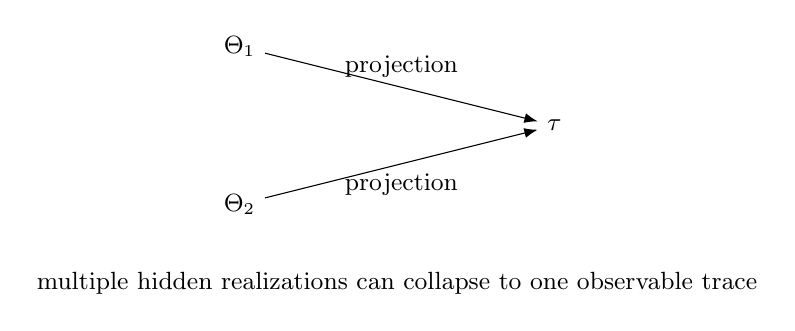
\begin{tikzpicture}[node distance=1.8cm, every node/.style={font=\small}]
\node (a0) at (0,2) {$\Theta_1$};
\node (a1) at (0,0) {$\Theta_2$};
\node (obs) at (4,1) {$\tau$};
\draw[-{Latex}] (a0) -- node[above] {projection} (obs);
\draw[-{Latex}] (a1) -- node[below] {projection} (obs);
\node at (2,-1) {multiple hidden realizations can collapse to one observable trace};
\end{tikzpicture}
\end{document}
